\section{Durchführung}

\subsection{Bestimmung der Widerstände}
Zuallererst wird der Widerstand von Kupfer und Zink bestimmt. Dafür werden Spulen aus den Materialien an eine Gleichstromquelle angeschlossen.
An dieser Gleichstromquelle lassen sich auch die Spannung und der Strom ablesen.
Anschließend wird parallel zu der Spule ein Voltmeter angeschlossen um die zum Strom korrespondierende abfallende Spannung zu messen.\\
Eine schematische Darstellung dieses Aufbaus ist in in Abb. \ref{img:hall} dargestellt.
\begin{figure}[H]
    \centering
    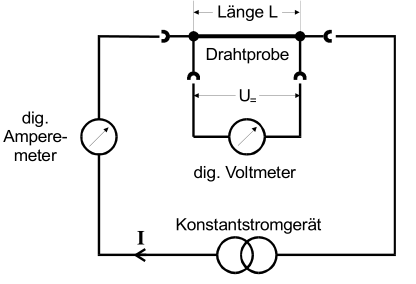
\includegraphics[width=0.55\textwidth]{images/widerstandmessung.PNG}
    \caption{Der Schaltplan für die Bestimmung des Widerstands\protect \cite{V311}.}
    \label{img:hall}
  \end{figure}
\noindent
Für diesen Aufbau werden dann diverse Messungen mit unterschiedlichen Stromstärken für Kupfer und Zink gemacht.\\
Des Weiteren werden, mit Hilfe eines digitalen Messschiebers, die Breite und Dicke zweier Metallplatten gemessen. Diese Platte sind denen, die zur Messung des Hall-Effektes genutzt werden, 
von ihren Ausmaßen sehr ähnlich.\\


\subsection{Hall-Effekt}
Die folgende Durchführung des Versuches wird für beide Metalle identisch durchgeführt.\\
Der Aufbau besteht aus zwei Spulen die parallel an ein Konstantstromgerät angeschloßen werden. 
Oben auf den Spulen sind zwei Metallblöcke, die von den Spulen magnetisiert werden und so zwischen ihnen ein annähernd homogenes Magnetfeld erzeugen.
In diesen Bereich lässt sich, auf eine Schiene, das zu untersuchende, auf einer Platte aufgebrachte, Substrat einführen\\
\begin{figure}[H]
    \centering
    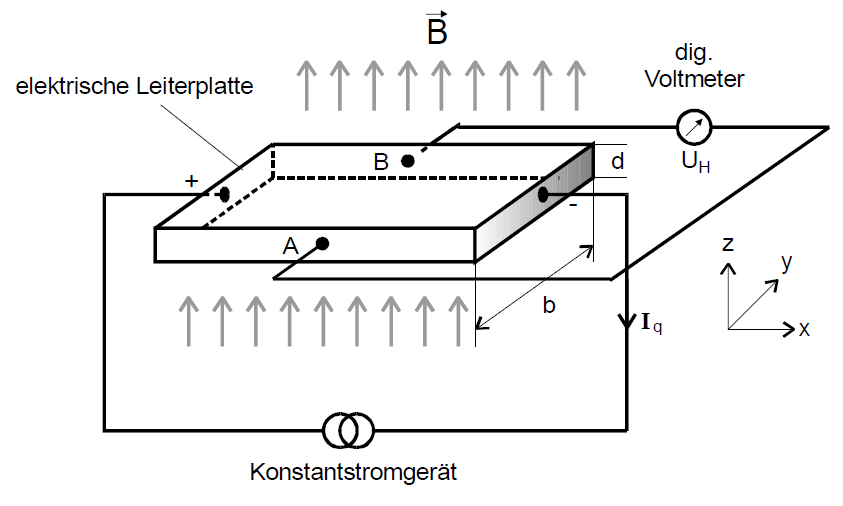
\includegraphics[width=0.45\textwidth]{images/hall.PNG}
    \caption{Der Schaltplan der Platte an der die Hall-Spannung gemessen wird \protect \cite{V311}.}
    \label{img:hall2}
  \end{figure}
\noindent
Die Platten mit den Substraten haben Anschlüsse, so dass sich an den Rändern des aufgebrachten Metalls die Hallspannung abgreifen lässt und so, 
dass sich zusätzlich ein Strom durch das Metall schicken lässt.
An der einen Seite der Platte wird also ein feines Voltmeter angeschloßen, um die Hallspannung abzugreifen und an dem anderen ein Konstantstromgerät.
Den Schaltplan die Platte betreffend ist in Abb.\ref{img:hall2} zu sehen.\\
Bevor die Hall-Spannung gemessen wird wird zuerst die Spule geeicht. Dies geschieht, in dem mit Hilfe einer Hallsonde, die zwischen den magnetisierten Metallen eingebracht wird,
das Magnetfeld für die später für das Magnetfeld genutzten Stromstärken gemessen wird.\\
Nun wird bei konstantem Magnetfeld der Stromfluss durch die Platte variiert und dabei die Hall-Spannung abgelesen.
Natürlich werden auch vom Konstantstromgerät die Stromstärken die durch die Platte und durch die Spule notiert.
Da die beiden Punkte an denen die Hall-Spannung abgegriffen wird keine Äquipotentialflächen seien müssen kann eine Spannungsabfall zwischen den beiden Punkten auftreten.
Dieser Spannungsabfall wird $U_\text{Stör}$ genannt. \\
Da diese Stör-Spannung bei konstantem Strom auch konstant ist lässt sie sich durch umpolen des Magnetfeldes herausrechnen.
\begin{align*}
  U_\text{ges+}&=U_\text{Hall}+U_\text{Stör}\\
  U_\text{ges-}&=-U_\text{Hall}+U_\text{Stör}\\
  U_\text{Hall}&=\frac{1}{2}(U_\text{ges+}-U_\text{ges-})
\end{align*}
Es muss aber unbedingt darauf geachtet werden, dass die Umpolung der Spulen nicht abrupt geschehen darf, sondern die Spulen erst heruntergeregelt werden müssen.
Ansonsten können Schäden an dem Konstantstromgerät auftreteten.\\
Als letztes wird dann noch einmal eine Messreihe mit konstantem Stromfluss und variierter Magnetfeldstärke durchgeführt, bei der auch immer umgepolt wird.
